\subsection{Censur og overvågning af internettet}
Udbredelsen af internettet, og dens anvendelighed til kommunikation, betød ikke blot en løsning af manges ønsker på forbindelse og deling. Det global samfund havde fundet en forholdsvis åben dør til en kiste fyldt, med alle de tænkelige informationer, kun få klik væk. Denne magt internettet pludselig fik over menneskers data betød også at en vækst af magtmisbrug af det internet, der var tiltænkt at skulle være åbent og frit.
\subsubsection{Hvem er Freedom House?}
Den globale internet frihed er på syvende år i træk stadig dalende\cite{FreedomHouseRapport2017}, lyder det fra den uafhængige frihedskæmpende organisation Freedom House i deres årlige rapport "Freedom on the Net". Freedom House har til formål at fremme frihed og demokrati rundt omkring i verden, blandt andet ved at fortage dybdegående analyser, og ved at være fortaler for menneskerettigheder.\cite{FreedomHouseAbout} De nyeste årlige "Freedom on the Net" rapporter fra 2016 og 2017, der dækker mindst 87\% af verdens internet benyttende befolkning, giver hvert år et resumé af hvilke trends der havde størst betydning for deres samlede konklusion. \\
\noindent
Hvert af de 65 lande der årligt bliver afdækket, får tildelt sig en numerisk score, alt efter hvor god eller ringe deres internet frihed har været. Denne score går fra 0 til 100, og er opdelt i 3 overordnet kategorier: Free, Partly Free og Not Free [Se Tabel: \ref{fig:freedomscale}].\\ 
En score er bestemt ud fra 3 overordnet kriterier: Forhindringer for adgangen til nettet, restriktioner på indholdet og overtrædelser af brugernes rettigheder [Se Tabel: \ref{fig:freedomscale2}].\cite{FreedomHouseRapportMethodology}
\\
\begin{table}[H]
    \begin{minipage}{.5\textwidth}
        \centering
        \begin{tabular}{|l|l|}
            \hline
            \textbf{Kategori} & \textbf{Points} \\ \hline
            Free              & 0 - 30          \\ \hline
            Partly Free       & 31 - 60         \\ \hline
            Not Free          & 61 - 100        \\ \hline
        \end{tabular}
        \caption{Freedom House frihedsskala}
        \label{fig:freedomscale}
    \end{minipage}
    \begin{minipage}{.5\textwidth}
        \centering
        \begin{tabular}{|l|l|}
            \hline
            \textbf{Kriterier}                     & \textbf{Points} \\ \hline
            Forhindringer for adgangen til nettet  & 0 - 25          \\ \hline
            Restriktioner på indholdet             & 0 - 35          \\ \hline
            Overtrædelser af brugernes rettigheder & 0 - 40          \\ \hline
        \end{tabular}
        \caption{Freedom House frihedsskala}
        \label{fig:freedomscale2}
    \end{minipage}
\end{table}

\subsubsection{Censur mod sociale medier}
I 2016 udgivelsen af rapporten, blev den stigende magtmisbrug af de sociale medier, samt andre kommunikationskanaler, belyst. I 2015 fandt Freedom House frem til, at 15 regeringer ud af de 65 undersøgte, havde begrænset befolkningens adgang til diverse sociale medier, i 2016 havde dette tal forøget sig til 24. Brasilien og Tyrkiet endte 2016's undersøgelse med, at blive to af de mest bemærkelsesværdige lande, da de begge gik et betydeligt skidt tilbage på deres respektive frihedsskalaer, netop på grund af deres magtanvendelse overfor diverse sociale medier. Brasilien gik fra kategorien "Free" til "Partly Free", da brasilianske domstole indførte en midlertidig blokering af opkald- og tekstkommunikations tjenesten WhatsApp. WhatsApp nægtede nemlig at udlevere brugerdata til bevismateriale.\\ 
Tyrkiet gik fra kategorien "Partly Free" til "Not Free" efter masseblokeringer af diverse sociale medier, og efterfølgende forfølgelse af borgere, der kritiserede Tyrkiets regering.\cite{FreedomHouseRapport2016}\\\\
\noindent
Den mest hyppige årsag til regeringers, især autoritære regimers, restriktioner af diverse sociale medier, er for at holde deres befolkninger i skak. Disse restriktioner sker blandt andet når en regering kritiseres, når der mistænkes korruption eller lignede. Gennem tiden har utilfredse bevægelser kunne samle sig og kæmpe for hvad de troede på, og dette har ført til blandt andet væltede monarker, arbejdsgivere og regimer. Det ses stadig i dag hvordan bevægelser kæmper rundt om i verden mod uretfærdighed, f.eks under Det Arabiske Forår hvor at en række arabiske lande gjorde op med deres diktatoriske ledelse.\cite{ArabiskeForaar} Under disse oprør, især i nyere tid, har de sociale medier været uvurderlige i at få befolkningsgrupper engageret og oplyst til at ville kæmpe for deres respektive sag. Da disse sociale medier er gode til at få samlet folk, og organisere protester og lignede, vil visse regeringer bruge deres magt på undertrykkelse. Det er dog ikke kun aktivisme, nogle af disse autoritære regimer undertrykker også homoseksuelle fællesskab, satire, religiøse- og modstående politiske overbevisninger. Disse udsatte grupper har i høj grad brug for at de kommunikationskanaler de benytter beskytter deres kommunikation og oplysninger, sådan de ikke falder i de forkerte hænder.

\subsubsection{Sikkerhed og privatlivet i fare}
Moderne efterforskning inkluderer i højere grad de forskellige kommunikationskanaler, når kriminalitet og terror aktivitet skal bekæmpes. Smartphone, computere og online services er i vor tid tætpakket med avanceret kryptering, både for at beskytte virksomhedens brugere, men også virksomheden selv. Denne kryptering så myndighederne, i blandt andet Kina, Ungarn, Rusland, Thailand, Storbritannien og Vietnam, gerne gradbøjet, som led i individuelle lov ændringer indefor området. Disse love kan blandt andet kræve at virksomheder udleverer backdoor eller bagdørs krypteringsnøgler til myndighedernes efterretningstjenester. Dette kan udgøre en kolossal risiko for alle brugerene af det pågældende medie, især for de brugere der har brug for en sikker kanal til journalistik, aktivisme osv.\cite{FreedomHouseRapport2017} Det åbner op for at visse regeringer har muligheden for at misbruge brugerne på de sociale mediers data udenfor et efterforsknings miljø, hvilket også er virksomhedernes største frygt i forbindelse med disse bagdøre.\\
\begin{figure}[H]
    \centering
    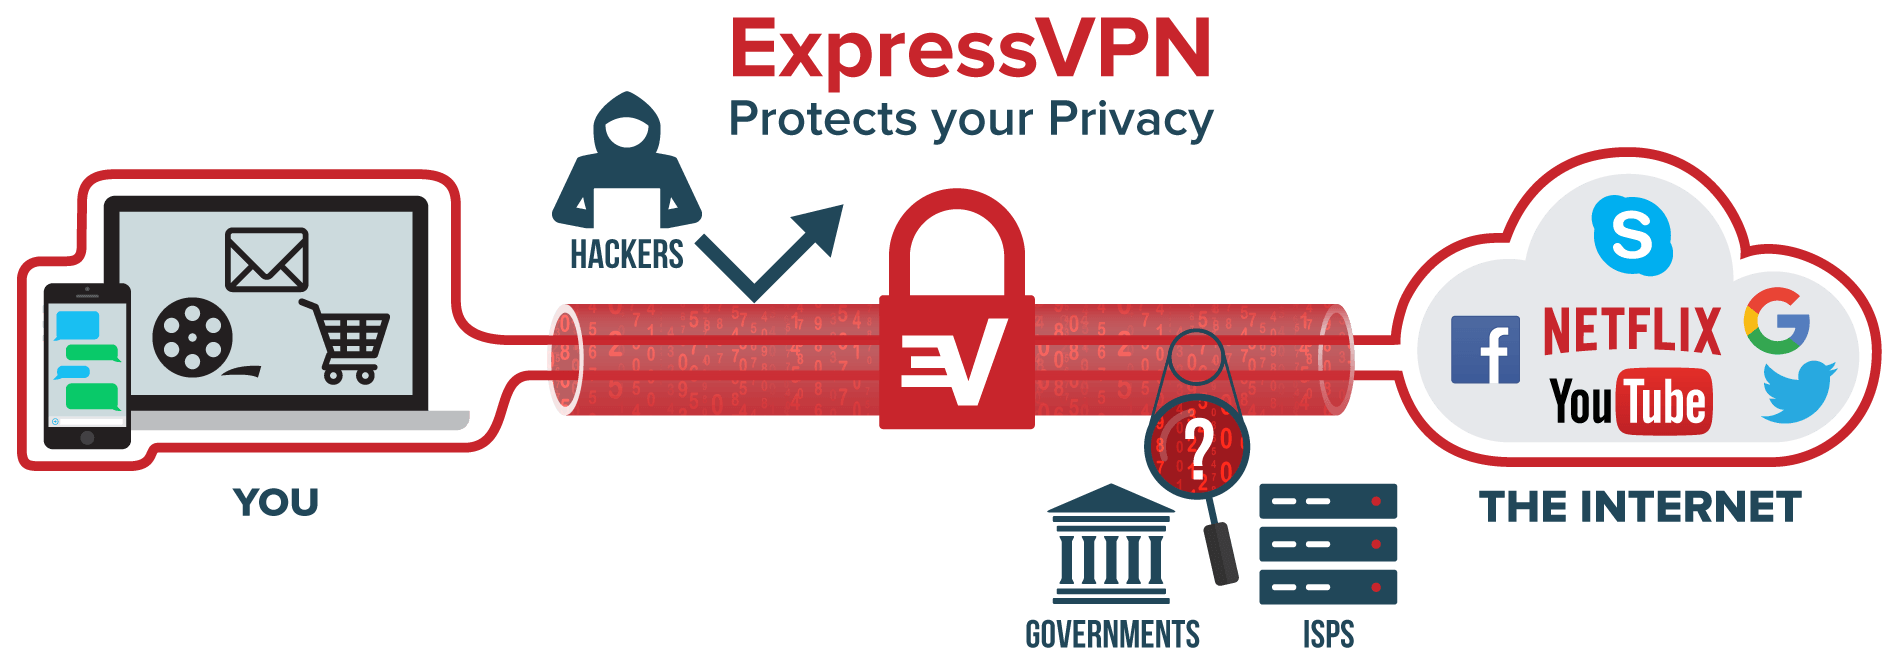
\includegraphics[scale=0.2]{Projectdoc/Problemanalyse/Illustrationer/vpn.png}
    \caption{En illustration fra ExpressVPN, der viser hvordan en VPN forbindelse ser ud på overfladen\cite{ExpressvpnImage}}
    \label{fig:vpn}
\end{figure}
\noindent
En anden sikkerhedsforanstaltning, som diverse regeringer, herunder Kina, Rusland og Egypten\cite{FreedomHouseRapport2017}, ønsker at regulere, er VPN'er eller Virtual Private Networks. En VPN beskytter brugerens privatliv og sikkerhed på nettet, ved at fungere som et ekstra led mellem brugerens enhed og internettet [Se Figur: \ref{fig:vpn}]. Denne forbindelse er krypteret, som betyder at brugerens data og handlinger er sikret.\cite{VPNInfo} Derudover kan en VPN virtuelt skifte den geografiske position af en given enhed, og dermed undgå eventuelle regeringers censur, af for eksempelvis internationale nyhedsbureauer, eller sociale medier. Selvom VPN kan blive brugt til kriminel aktivitet, så bruger de fleste den til godsindet formål, såsom: at værne om privatlivet, forblive informeret via censureret medier, eller blot som et led i deres internationale arbejde. De regeringer der ønsker at regulere VPN'er, vil dog ikke blokerer VPN'erne helt, da de netop bruges af regeringens ansatte, som et essentielt redskab. Regeringerne ønsker en proces, hvor at den enkelte VPN udbyder skal autoriseres til at operere i et given land, ved et sæt defineret brugstilfælde, resten af udbyderne vil blive blokeret af regeringen.\cite{FreedomHouseRapport2017}
